\chapter{Logistic Regression and Regularization}

Now we turn away from regression to classification problems. Don't be confused by the name `logistic regression,' it's actually just named for the mathematical function and it's a common approach to classification.

\section{Binary Classification}
In classification problems, instead of our output being continuous, we expect it to fall into discrete classes. We'll start with the simplest case: binary classification. Here, we have our output variable $y \in \{0, 1\}$. Typically, we take $0$ as the negative class and $1$ as the positive class. 

Consider the following example: we have a sample of eight tumors, and we want to determine if they're malignant based on the tumor size. These are plotted in Figure \ref{logreg-eg-maltumor-noregline}. One thing we can do is assume a linear relationship with hypothesis $h_\theta\left( \vec{x} \right) = \vec{\theta}^\intercal \vec{x}$. This shown in Figure \ref{logreg_eg1_maltumor_linreg1}.

\begin{figure}[h]
	\centering
	\begin{subfigure}[t]{0.45\textwidth}
   		\centering
    		\graphicspath{{./Figures/}}
  		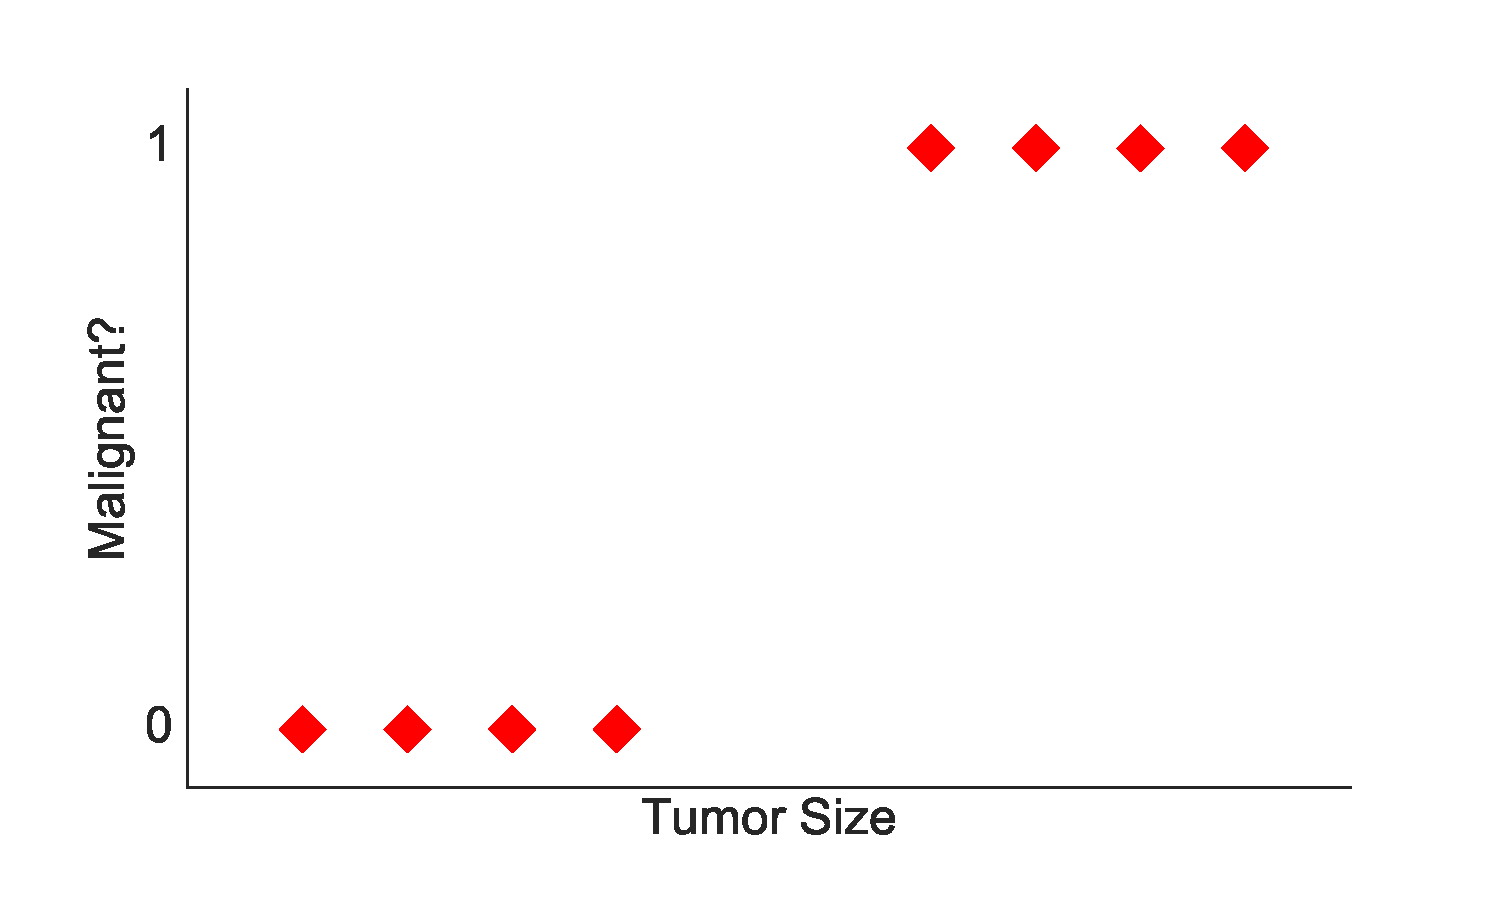
\includegraphics[scale=0.3]{logreg_eg1_maltumor.pdf} 
   		\caption[]{Sample tumor data.}
   		\label{logreg-eg-maltumor-noregline}
	\end{subfigure}
	\begin{subfigure}[t]{0.45\textwidth}
   		\centering
    		\graphicspath{{./Figures/}}
   		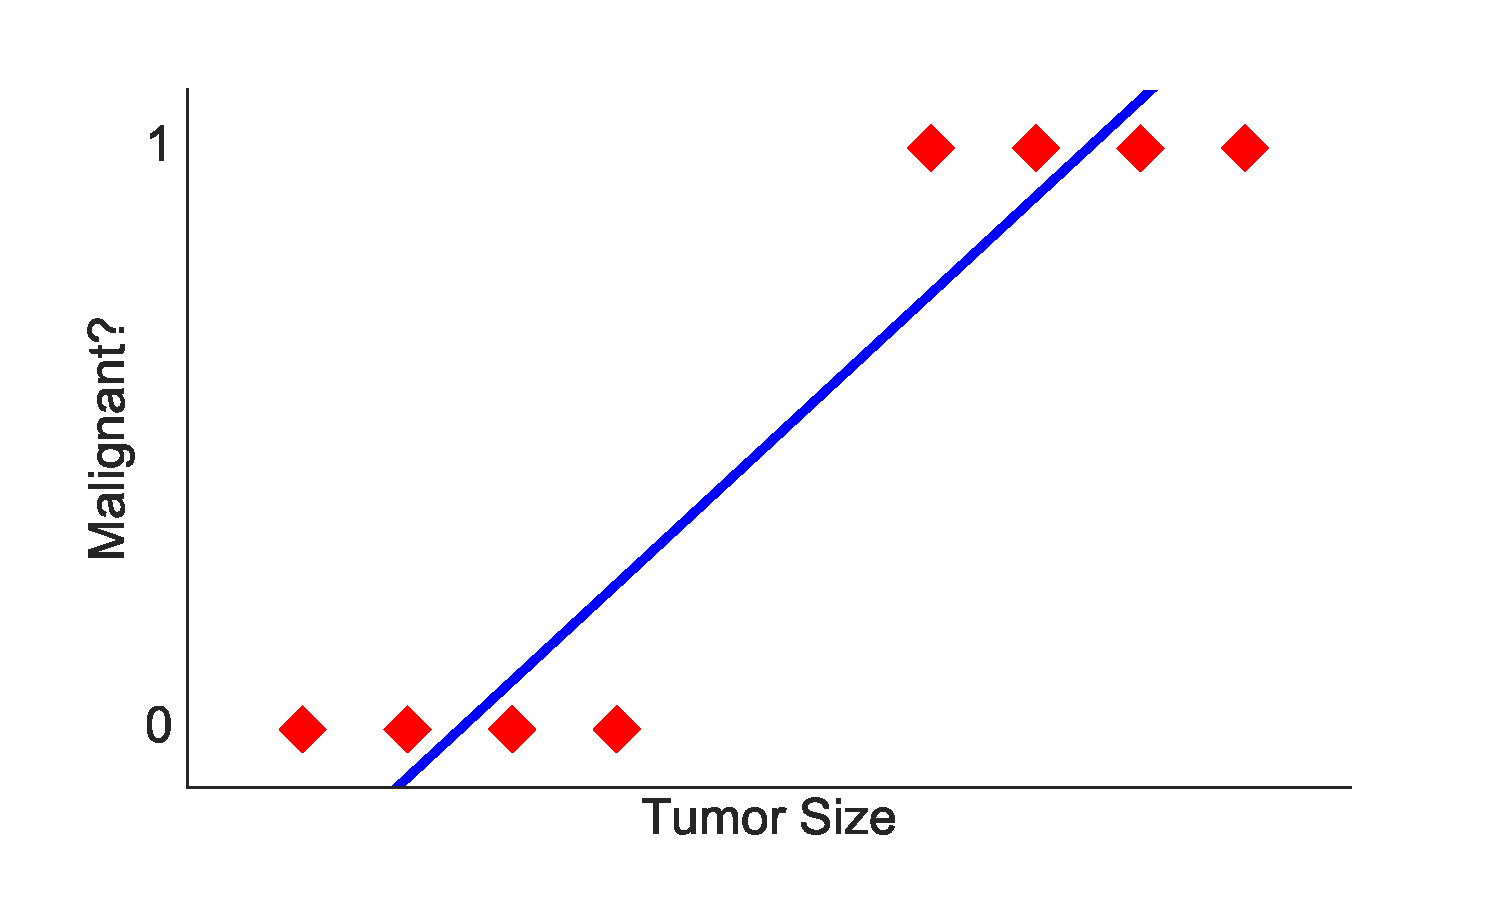
\includegraphics[scale=0.3]{logreg_eg1_maltumor_linreg1.pdf} 
   		\caption[]{Plot of tumors by size with linear regression line $y =  \frac{x-1}{6} - 0.25$.}
   		\label{logreg_eg1_maltumor_linreg1}
	\end{subfigure}
	\caption[]{Plots of tumors by size.}
\end{figure}

To try and make predictions, we can threshold the output at $h_\theta\left( x \right) = 0.5$, and then:
\begin{itemize}
\item If $h_\theta\left(x\right) \geq 0.5$, then predict $y = 1$
\item If $h_\theta\left( x \right) < 0.5$, then predict $y = 0$
\end{itemize}
and you can see this in Figure \ref{logreg_eg1_maltumor_linreg1_threshold.pdf}.

\begin{figure}[h] 
	\centering
	\graphicspath{{./Figures/}} 
	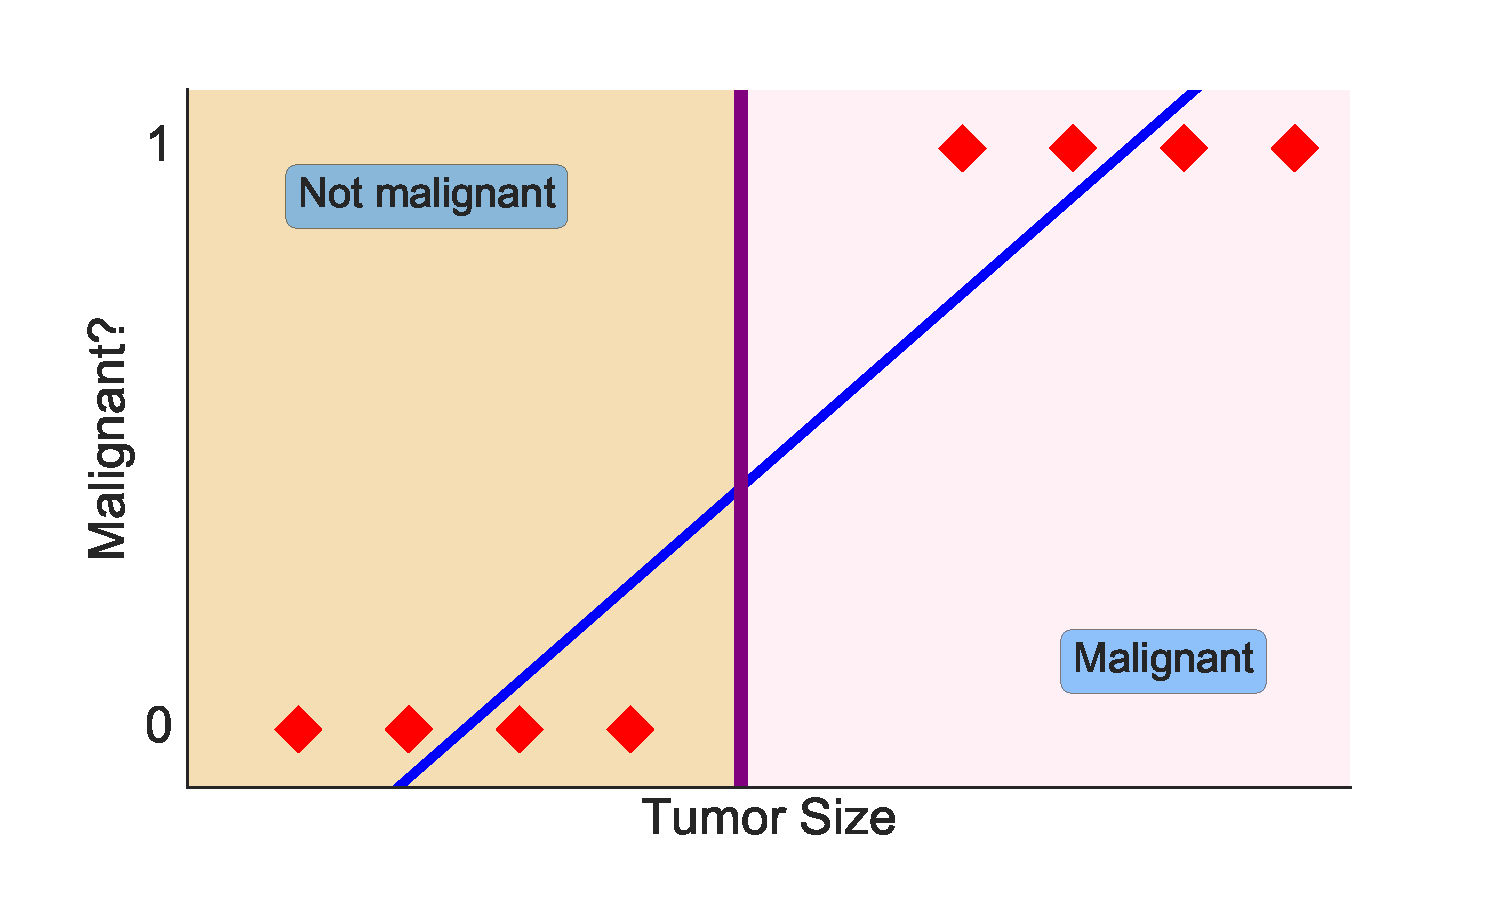
\includegraphics[scale=0.4]{logreg_eg1_maltumor_linreg1_threshold.pdf} 
	\caption[]{Linear regression plotted with classification regions. }
	\label{logreg_eg1_maltumor_linreg1_threshold.pdf}
\end{figure}


In this example, it would seem like linear regression is a good classifier. However, what if we add a new data point for a large tumor. Suddenly, our results look like this

\begin{figure}[h] %  figure placement: here, top, bottom, or page
	\centering
	\graphicspath{{./Figures/}} %Use this to import an image from a subfolder.
	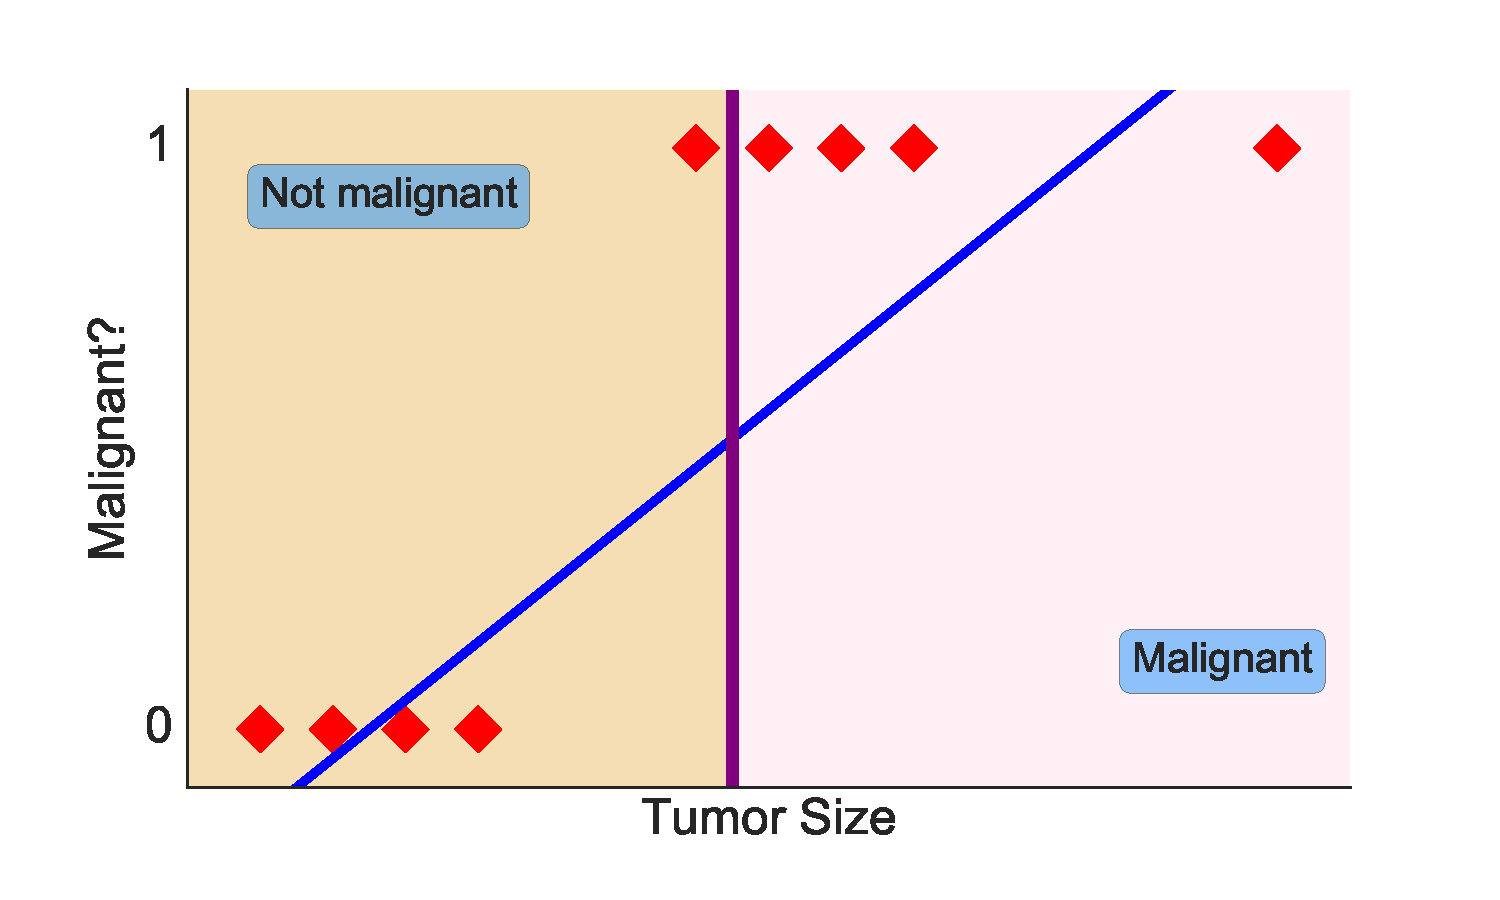
\includegraphics[scale=0.4]{logreg_eg1_maltumor_linreg1_newpoint.pdf} 
	\caption[]{Linear regression plotted with classification regions after a new data point is added. Notice how one of the malignant tumors is now being misclassified as benign.}
	\label{logreg_eg1_maltumor_linreg1_newpoint.pdf}
\end{figure}

and now, we have a malignant tumor being misclassified as benign. Ergo, maybe linear regression isn't the best way to build a binary classifier. 






\section{Hypothesis Representation}
In linear regression, our hypothesis was $h_\theta\left(\vec{x}\right) = \vec{\theta}^\intercal \vec{x}$ For logistic regression, we want our hypothesis to satisfy $0 \leq h_\theta\left(x\right) \leq 1$. To do this, we use the sigmoid function.\footnote{This is also called the logistic function, and is the namesake for logistic regression.} To make this work, we modify our hypothesis to be
\begin{equation}
h_\theta\left(x\right) = g\left(\vec{\theta}^\intercal \vec{x}\right)
\end{equation}
where the function $g\left(z\right)$ is defined as
\begin{equation}
g\left(z\right) = \frac{1}{1 + e^{-z}}
\end{equation}
Thus, to get the hypothesis function using the sigmoid function, just set $z = \vec{\theta}^\intercal \vec{x}$. 

The sigmoid function, shown in Figure \ref{logreg_eg2_sigmoid_func_plot.pdf}, maps any real number onto the interval $\left(0, 1\right)$. This makes it immensely useful for transforming an arbitrary function for use with classification.


\begin{figure}[h] %  figure placement: here, top, bottom, or page
	\centering
	\graphicspath{{./Figures/}} %Use this to import an image from a subfolder.
	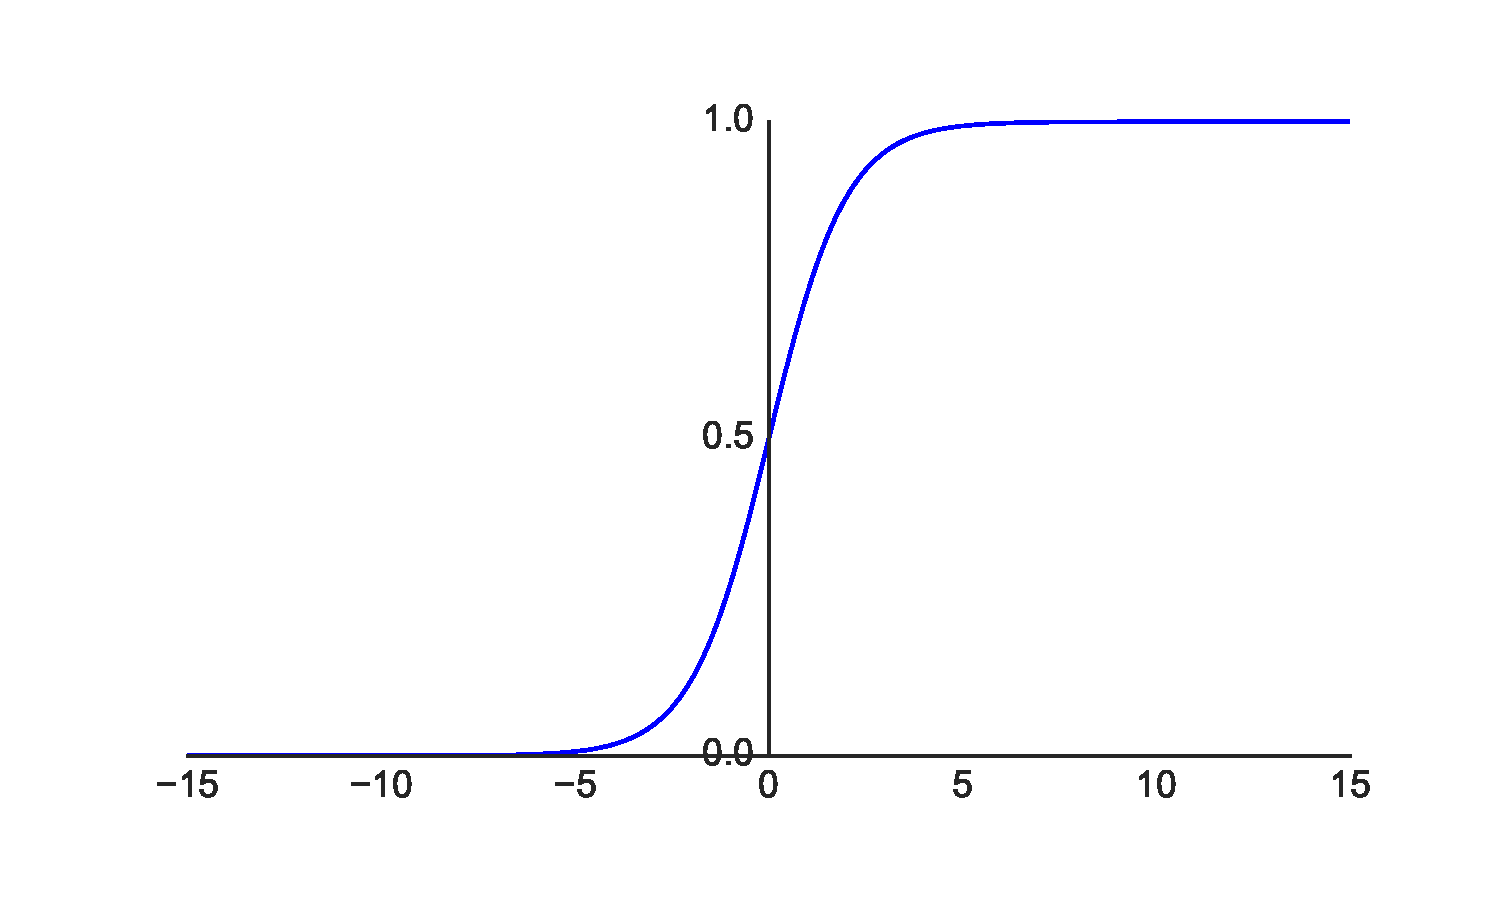
\includegraphics[scale=0.4]{logreg_eg2_sigmoid_func_plot.pdf} 
	\caption[]{Sample plot of the sigmoid function.}
	\label{logreg_eg2_sigmoid_func_plot.pdf}
\end{figure}


\subsection{Interpretation of the Logistic Hypothesis Function}

When examining the hypothesis function output for logistic regression, we interpret $h_\theta\left(x \right)$ is the estimated probability that $y=1$ on an input example $x$. For example, let's revisit the tumor size question from above. We have 
$$
\vec{x} = \left[\begin{array}{c}x_0 \\ x_1 \end{array}\right] = \left[\begin{array}{c}1 \\ \text{tumor size} \end{array}\right]
$$
If our hypothesis $h_\theta\left( x \right) = 0.7$, then we can tell the patient that there is a 70\% chance of the tumor being malignant. 

Slightly more formally, we interpret $h_\theta\left(x\right)$ as:\footnote{This is read as "the probability that $y = 1$, given $x$, parameterized by $\theta$.}
\begin{equation}
h_\theta\left(x\right) = P\left(y=1 | x; \theta\right)
\end{equation}
Thus, by the rules of probability:
\begin{align}
P\left(y=0 | x; \theta\right) + P\left(y=1 | x; \theta\right) = 1 \\
P\left(y=0 | x; \theta\right) = 1 - P\left(y=1 | x; \theta\right)
\end{align}


\subsection{Fitting Logistic Regression to a Binary Classifier}
\label{chaplogreg-sect-hyporeg-subsectbinclasfit}
Now, we need to fit our hypothesis function into a binary classfier: $0$ or $1$. Using our probabilistic interpretation of the logistic hypothesis function, we can make the following supposition:

\begin{align}
y  = 1 &\text{ given that } h_\theta\left(x\right) \geq 0.5 \\
y = 0 &\text{ given that } h_\theta\left(x\right) < 0.5
\end{align}

Recall the plot of the sigmoid function in Figure \ref{logreg_eg2_sigmoid_func_plot.pdf}. We see that $g\left(z\right) \geq 0.5$ when $z \geq 0$. In our case, if we're setting $z = \vec{\theta}^\intercal \vec{x}$, then we have:

\begin{equation}
h_\theta\left(x\right) = g\left(\vec{\theta}^\intercal\vec{x}\right) \geq 0.5 ~~\mbox{ when }~~ \vec{\theta}^\intercal\vec{x} \geq 0
\end{equation}

\noindent From this, we can now state
\begin{align}
\vec{\theta}^\intercal\vec{x} \geq 0 &\implies y = 1 \\
\vec{\theta}^\intercal\vec{x} < 0 &\implies y= 0
\end{align}

\noindent When utilizing the sigmoid function, keep the following in mind:
\begin{itemize}
\item When $z = 0$, then $e^0 = 1$ so $g\left(x\right) = \frac{1}{2}$
\item When $z$ goes to $\infty$, we have $e^{-\infty} \to 0$, and this implies $g\left(x\right) = 1$
\item As $z \to -\infty$, $e^\infty \to \infty \implies g\left(z\right) = 0$
\end{itemize}


\section{Decision Boundary}
\begin{figure}[h] %  figure placement: here, top, bottom, or page
	\centering
	\graphicspath{{./Figures/}} %Use this to import an image from a subfolder.
	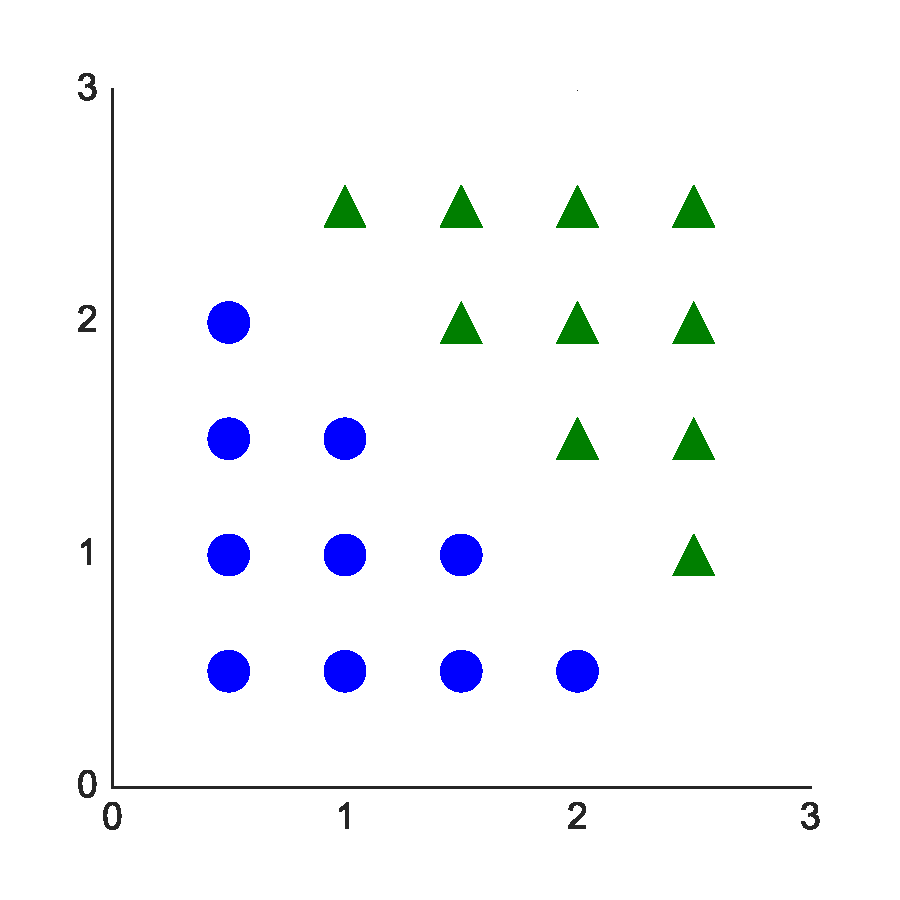
\includegraphics[scale=0.4]{logreg_eg3_decision_bndy_noline.pdf} 
	\caption[]{Sample data.}
	\label{logreg_eg3_decision_bndy_noline.pdf}
\end{figure}

Consider the data plotted in Figure \ref{logreg_eg3_decision_bndy_noline.pdf}. Suppose our hypothesis is given by
$$
h_\theta\left(x\right) = g\left(\theta_0 + \theta_1x_1 + \theta_2x_2\right)
$$
We haven't yet discussed how to fit the parameters of this model (that's coming up next), but suppose we choose the following values for the parameters
$$
\vec{\theta} = \left[\begin{array}{c}\theta_0 \\ \theta_1 \\ \theta_2\end{array}\right] = \left[\begin{array}{c} -3 \\ 1 \\ 1 \end{array}\right]
$$

Given this choice of parameters, let's figure out where $y=1$ and where $y=0$. From \S\ref{chaplogreg-sect-hyporeg-subsectbinclasfit}, recall that we predict $y=1$ when $\vec{\theta}^\intercal\vec{x} \geq 0$, so here, we predict $y=1$ if $-3 + x_1 + x_2 \geq 0$. If we solve this for $x_1 + x_2$ we get
$$
x_1 + x_2 \geq 3 \implies y = 1
$$
If we change this to a pure equality, $x_1 + x_2 = 3$, we have the equation of a straight line (shown on Figure \ref{logreg_eg3_decision_bndy_withline.pdf}). The line drawn, is called the \textbf{decision boundary}. The decision boundary is the line created by the hypothesis function that separates the area where we classify $y=0$ and where $y=1$.

\begin{figure}[h] %  figure placement: here, top, bottom, or page
	\centering
	\graphicspath{{./Figures/}} %Use this to import an image from a subfolder.
	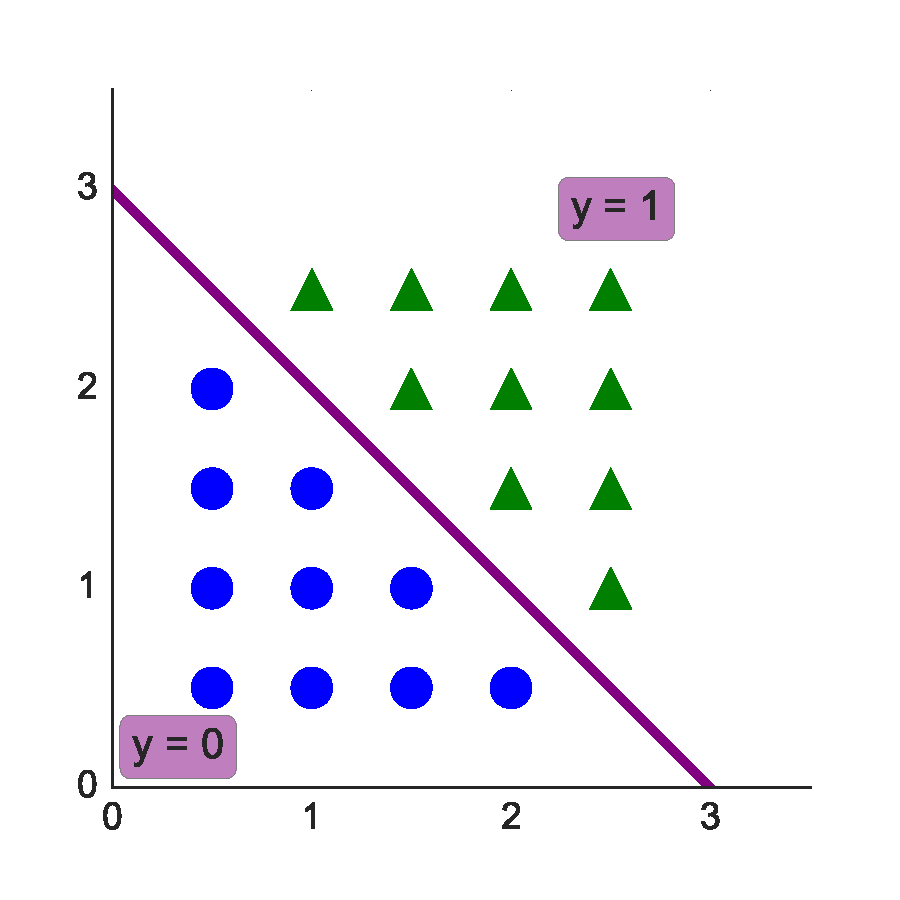
\includegraphics[scale=0.4]{logreg_eg3_decision_bndy_withline.pdf} 
	\caption[]{Some sample binary data with a plotted decision boundary. Here, the blue circles represent $y=0$, the green triangles $y=1$ and the purple line is the decision boundary.}
	\label{logreg_eg3_decision_bndy_withline.pdf}
\end{figure}

To be clean, the decision boundary is a property of the hypothesis function, and not a property of the dataset. We fit the parameters of the hypothesis based on the training data, but once those parameters are set, the decision boundary is a property solely of the hypothesis function. 

Now, suppose we have data as shown below in Figure \ref{logreg_eg3_decision_bndy_nonlinear_nocirc.pdf}. It's fairly obvious that no straight line decision boundary will work for this data. Again, we don't know how to fit the parameters for this model yet, but say our hypothesis function looks like this
$$
h_\theta\left(x\right) = g\left(\theta_0 + \theta_1x_1 + \theta_2x_2 + \theta_3x_1^2 + \theta_4x_2^2\right)
$$
Imagine we fit the parameters appropriately, and we get
$$
\vec{\theta} = \left[\begin{array}{c} \theta_0 \\ \theta_1 \\ \theta_2 \\ \theta_3 \\ \theta_4 \end{array}\right] = \left[\begin{array}{c}-1 \\ 0 \\ 0 \\ 1 \\ 1 \end{array}\right]
$$
Then, our hypothesis predicts that $y=1$ when $x_1^2 + x_2^2 \geq 1$. This is the equation for a circle of radius $1$, centered at the origin (see Figure \ref{logreg_eg3_decision_bndy_nonlinear.pdf}).
\begin{figure}[h]
	\centering
	\begin{subfigure}[t]{0.45\textwidth}
   		\centering
    		\graphicspath{{./Figures/}}
  		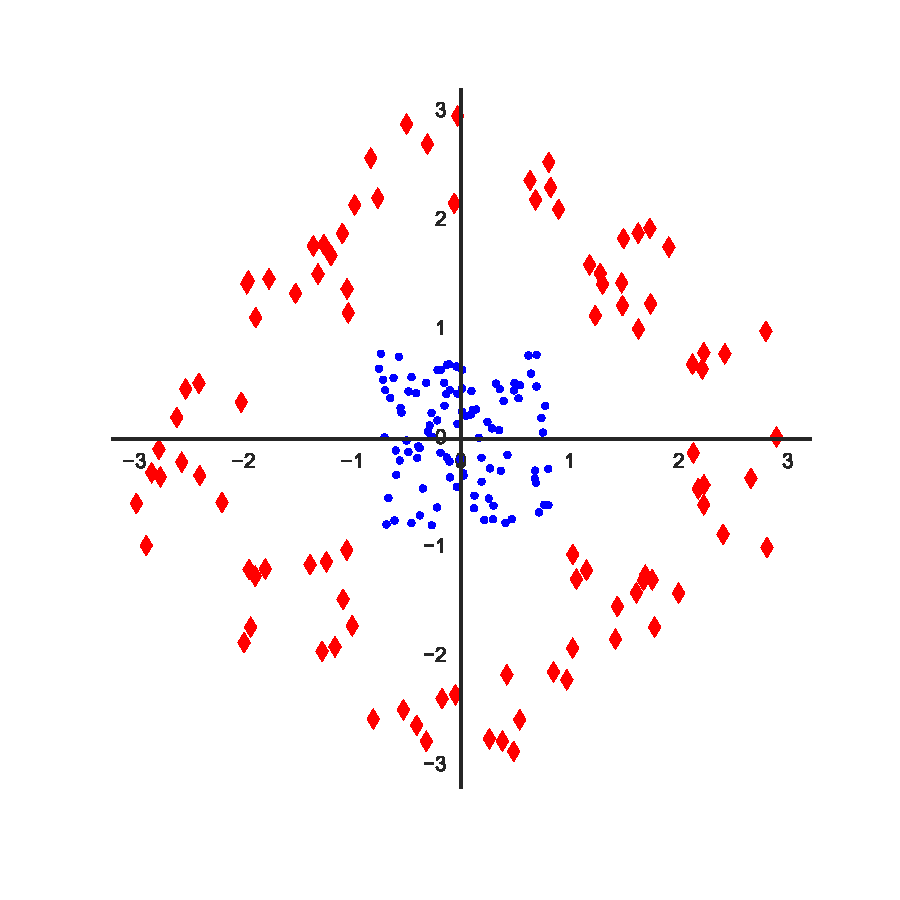
\includegraphics[scale=0.4]{logreg_eg3_decision_bndy_nonlinear_nocirc.pdf} 
   		\caption[]{This is a sample of data with no clear linear decision boundary.}
   		\label{logreg_eg3_decision_bndy_nonlinear_nocirc.pdf}
	\end{subfigure}
	\begin{subfigure}[t]{0.45\textwidth}
   		\centering
    		\graphicspath{{./Figures/}}
   		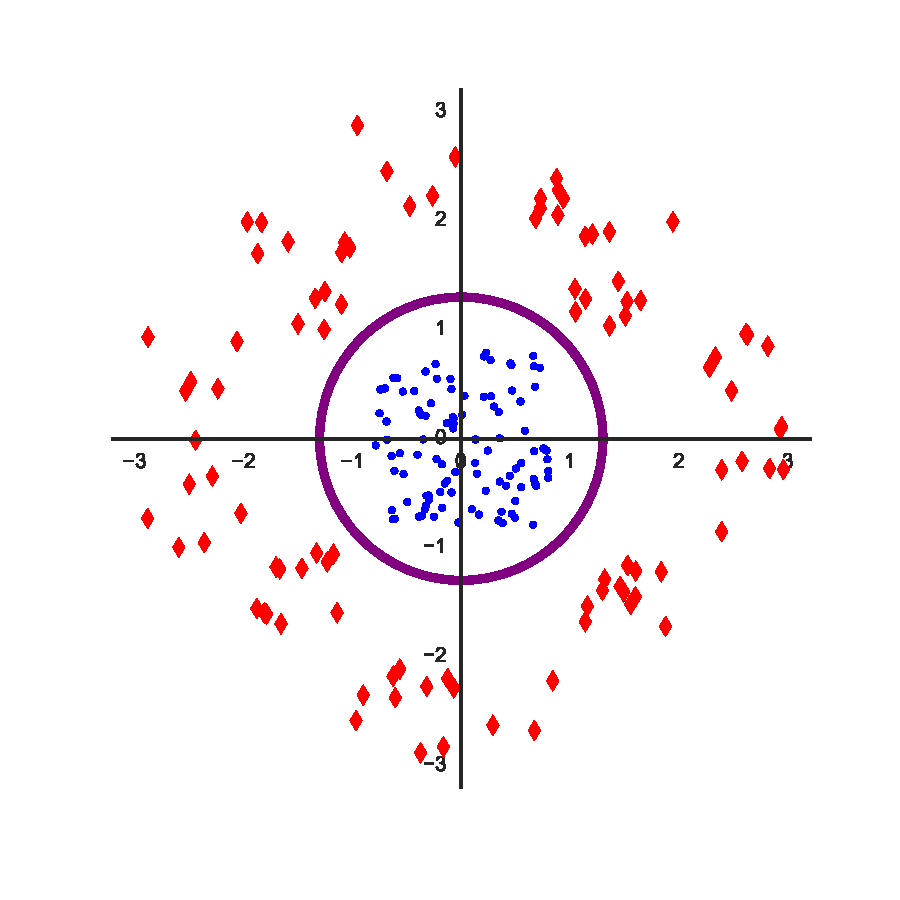
\includegraphics[scale=0.4]{logreg_eg3_decision_bndy_nonlinear.pdf} 
   		\caption[]{By altering our hypothesis function to include polynomial terms, we can have a non-linear decision boundary.}
   		\label{logreg_eg3_decision_bndy_nonlinear.pdf}
	\end{subfigure}
	\caption[]{Data that can't be fit with a linear decision line.}
\end{figure}
In this case, we predict $y=1$ everywhere outside the purple circle, and $y=0$ everywhere inside the circle. 

With even higher order polynomials, we can get even more complicated decision boundaries. 


\section{Cost Function}
Imagine we have a training set of data with $m$ examples
$$
\left\{ \left(x^{\left(1\right)}, y^{\left(1\right)}\right), \left(x^{\left(2\right)}, y^{\left(2\right)}\right), \cdots, \left(x^{\left(m\right)}, y^{\left(m\right)}\right) \right\}
$$
and $n$ features, represented by an $n+1$-dimensional feature vector
$$
x \in \left[\begin{array}{c} x_0 \\ x_1 \\ \vdots \\ x_n \end{array}\right]
$$
where $x_0 = 1$ and our output $y \in \{0, 1\}$. Our hypothesis is given by
\begin{equation}
h_\theta\left(x\right) = \frac{1}{1 + e^{-\theta^{{}^\intercal}x}}
\end{equation}
How do we choose the parameters for this model? For linear regression, we had the following cost function (adjusted slightly, we moved the $\tfrac{1}{2}$ to the inside of the summation)
\begin{equation}
J\left(\theta\right) = \frac{1}{m} \sum_{i=1}^m \frac{1}{2} \left(		h_\theta\left(x^{\left(i\right)}\right) - y^{\left(i\right)}	\right)^2
\end{equation}
but we're going to change how we write this function a little bit. Instead, we'll write
\begin{equation}
J\left(\theta\right) = \frac{1}{m} \sum_{i=1}^m \text{Cost}\left(	h_\theta\left(x^{\left(i\right)}\right), y^{\left(i\right)}\right)
\end{equation}
where we'll define the cost to be
\begin{equation}
\text{Cost}\left(	h_\theta\left(x^{\left(i\right)}\right), y^{\left(i\right)}\right) = \frac{1}{2} \left(h_\theta\left(x^{\left(i\right)}\right) - y^{\left(i\right)}	\right)^2
\end{equation}
This allows us to see more clearly that the cost function is really the sum over the cost term. To simplify even further, we'll remove the superscripts $\left(i\right)$
\begin{equation}
\text{Cost}\left(h_\theta\left(x\right), y\right) = \frac{1}{2} \left(	h_\theta\left(x\right) - y \right)^2
\end{equation}


If we try to minimize this function called Cost, it turns out to be a non-convex function. That means that the may be several local minima, which would prevent our gradient descent algorithm from working well. You can see a sample non-convex function in Figure \ref{logreg_eg4_sample_nonconvex_curve.pdf}. What we want instead, is a convex function (like a parabola) that only has a single minimum that is the global minimum. The sigmoid function is a non-linear signal function, so $J\left(\theta\right)$ ends up being non-convex. 
\begin{figure}[h] %  figure placement: here, top, bottom, or page
	\centering
	\graphicspath{{./Figures/}} %Use this to import an image from a subfolder.
	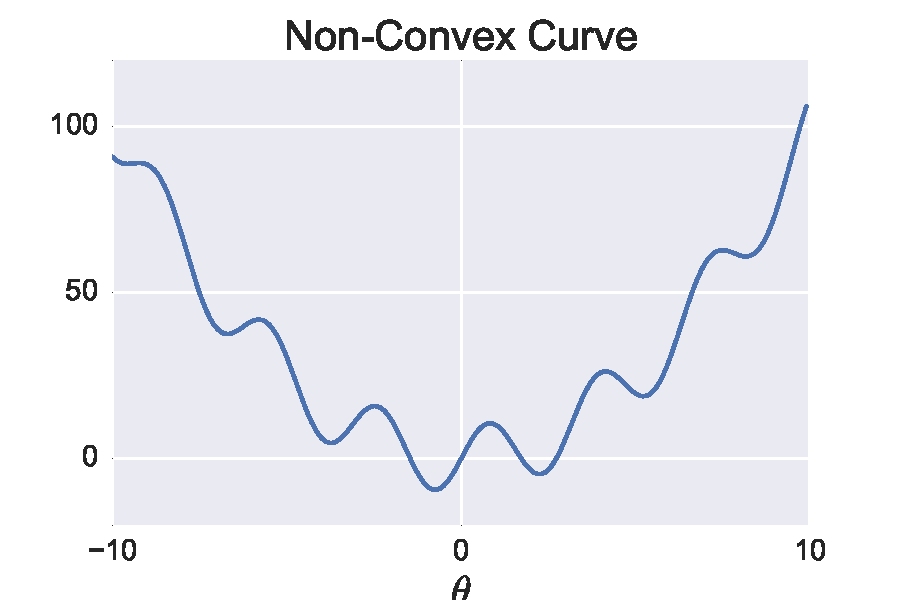
\includegraphics[scale=0.6]{logreg_eg4_sample_nonconvex_curve.pdf} 
	\caption[]{A non-convex curve. Notice all of the local minima.}
	\label{logreg_eg4_sample_nonconvex_curve.pdf}
\end{figure}

We need to define a new (convex) function that will allow us to determine the parameters in our hypothesis. For logistic regression, we use the following function
\begin{equation}
\text{Cost}\left(h_\theta\left(x\right), y\right) = \begin{cases} -\log\left(h_\theta\left(x\right)\right) & \text{if } y = 1 \\ -\log\left(1 - h_\theta\left(x\right)\right) &\text{if } y = 0 \end{cases}
\end{equation}
We plot this function below in Figure \ref{chaplogreg-sectcostfunct-plotcostfuncsample}. 

\begin{figure}[h]
	\centering
	\begin{subfigure}[t]{0.45\textwidth}
   		\centering
    		\graphicspath{{./Figures/}}
  		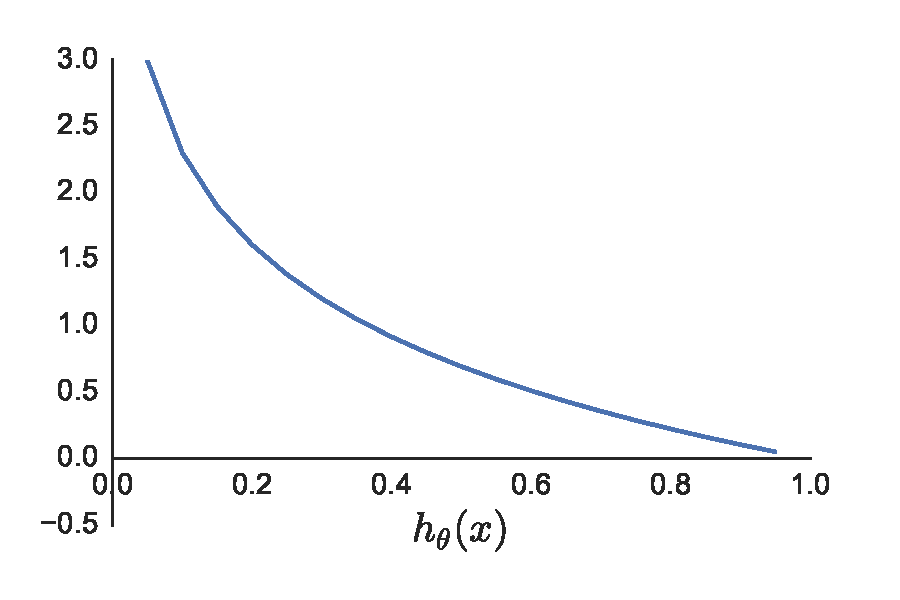
\includegraphics[scale=0.5]{logreg_eg5_cost_func_y1.pdf} 
   		\caption[]{$y=1$.}
   		\label{logreg_eg5_cost_func_y1.pdf}
	\end{subfigure}
	\begin{subfigure}[t]{0.45\textwidth}
   		\centering
    		\graphicspath{{./Figures/}}
   		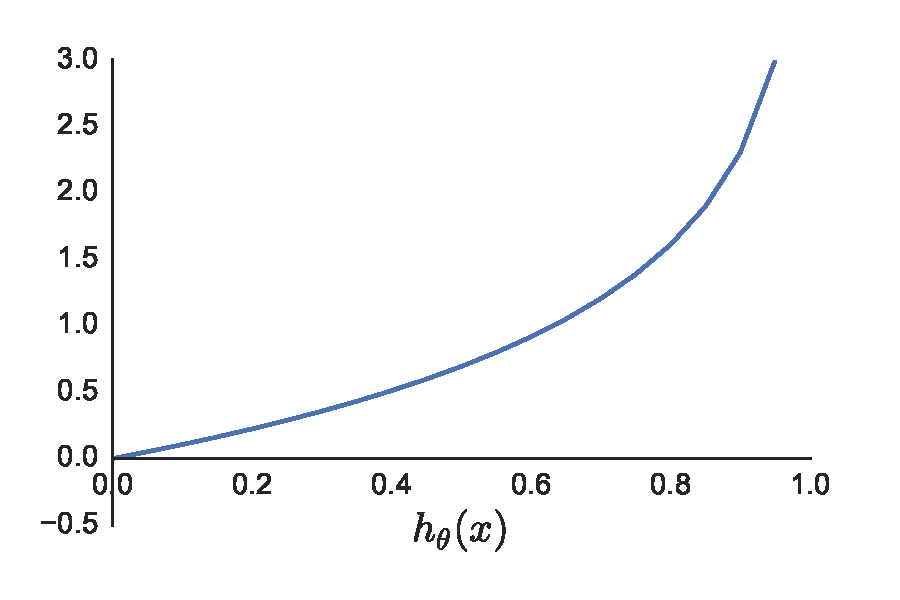
\includegraphics[scale=0.5]{logreg_eg5_cost_func_y0.pdf} 
   		\caption[]{$y=0$}
   		\label{logreg_eg5_cost_func_y0.pdf}
	\end{subfigure}
	\caption[]{The piecewise function used for the logistic regression cost function. }
	\label{chaplogreg-sectcostfunct-plotcostfuncsample}
\end{figure}

The shape of the curve comes from standard plot of $\log\left(x\right)$, and we just use a negative to flip it upside-down. This function, has some very desirable properties for us right now. 


\noindent \begin{minipage}{\linewidth}
\begin{itemize}
\item If $y = 1$, then $h_\theta\left(x\right) = 1$ and the cost is zero. However, as $h_\theta\left(x\right) \to 0$ then $\text{cost} \to \infty$. This captures the intuition that if $h_\theta\left(x\right) = 0$, but $y=1$, we'll penalize the learning algorithm by a very large cost. 
\item For $y=0$, this is reversed. If we have $y=0$ and $h_\theta\left(x\right) = 0$, then the cost is $0$. If $y=0$, the cost grows very large as $h_\theta\left(x\right)$ increases towards $1$. 
\end{itemize}
\end{minipage}


\subsection{Simplified Cost Function}
Recall our cost function 
\begin{equation}
J\left(\theta\right) = \frac{1}{m} \sum_{i=1}^m \text{Cost}\left(	h_\theta\left(x^{\left(i\right)}\right), y^{\left(i\right)}\right)
\end{equation}
where the cost is 
\begin{equation}
\text{Cost}\left(h_\theta\left(x\right), y\right) = \begin{cases} -\log\left(h_\theta\left(x\right)\right) & \text{if } y = 1 \\ -\log\left(1 - h_\theta\left(x\right)\right) &\text{if } y = 0
\end{cases}
\end{equation}
and $y \in \{0, 1\}$. 
Since $y$ is always either $0$ or $1$, we can take advantage of this to write a simplified version of our cost function:
\begin{equation}
\text{Cost}\left(h_\theta\left(x\right), y\right) = -y\log\left(h_\theta\left(x\right)\right) - \left( 1-y \right) \log\left(1 - h_\theta\left(x\right)\right)
\end{equation}
For either value of $y$, one of the terms will be multiplied by zero and disappear. So now, our cost function is\footnote{Just as an FYI, this cost function is derived statistically using maximum likelihood estimation}
\begin{align}
J\left(\theta\right) &= \frac{1}{m} \sum_{i=1}^m \text{Cost}\left(	h_\theta\left(x^{\left(i\right)}\right), y^{\left(i\right)}\right) \nonumber \\
\label{chaplogreg-sectsimpcostfunct-simpcostfuncformula}
&= -\frac{1}{m} \left[ \sum_{i=1}^m y^{\left(i\right)} \log h_\theta\left(x^{\left(i\right)}\right) + \left(1 - y^{\left(i\right)}\right) \log \left(1 - h_\theta\left(x^{\left(i\right)}\right)\right)\right]
\end{align}
We want to minimize the cost function$J\left(\theta\right)$ to fit the parameters $\theta$, so we can make our predictions using the hypothesis function. Again, we determine $\theta$ by calculating 
$$
\min_\theta J\left(\theta\right) 
$$
and predict using 
$$
h_\theta\left(x\right) = \frac{1}{1 + e^{\theta^{{}^\intercal}x}}
$$
using the calculated parameters. Now, we just need to determine how to minimize $J\left(\theta\right)$. 

\subsection{Gradient Descent for Logistic Regression}

We again return to gradient descent, of the form 


\textbf{Repeat until convergence:}
\begin{equation}
\theta_j := \theta_j - \alpha \frac{\partial}{\partial \theta_j} J\left( \theta \right)
\end{equation}
where we simultaneously update all $\theta_j$. If we calculate the partial derivative $\frac{\partial}{\partial \theta_j} J\left(\theta\right)$, we find
\begin{equation}
\frac{\partial}{\partial \theta_j} J\left(\theta\right) = \frac{1}{m}\sum_{i=1}^m \left( h_\theta\left(x^{\left(i\right)}\right) - y^{\left(i\right)}\right) x_j^{\left(i\right)}
\end{equation}
Plugging this back into the formula for gradient descent, we get


\textbf{Repeat until convergence:}
\begin{equation}
\theta_j := \theta_j - \frac{\alpha}{m} \sum_{i=1}^m \left( h_\theta\left(x^{\left(i\right)}\right) - y^{\left(i\right)}\right) x_j^{\left(i\right)}
\end{equation}
But wait! This looks exactly like the formula for linear regression! Is this actually a different algorithm? Yes! It is! The difference here is that the hypothesis function $h_\theta\left(x\right)$ is a different function. 

Remember that for gradient descent, we often need to apply feature scaling to make the algorithm run faster. 


\section{Vectorized Equations}
In equation \ref{chaplogreg-sectsimpcostfunct-simpcostfuncformula}, we derived a simplified version of the cost function. We can do the same thing with a vectorized implementation. First, we state the vectorized hypothesis function as
\begin{equation}
h = g\left( X\vec{\theta}\right)
\end{equation}
and then we can write the simplified cost function as
\begin{equation}
J\left(\theta\right) = \frac{1}{m}\cdot \left( -\vec{y}^\intercal \log\left(h\right) - \left(1 - \vec{y}\right)^\intercal \log \left(1 - h\right)\right)
\end{equation}


\section{Advanced Optimization}

There are other, more sophisticated algorithms that are able to more quickly optimize $\theta$. These algorithms are a little more complicated, so you shouldn't try to write them yourself unless you're an expert in numerical computing. 

In particular, there are three algorithms that we'll mention:
\begin{itemize}
\item Conjugate gradient algorithm
\item Broyden-Fletcher-Goldfarb-Shanno (BFGS) algorithm
\item L-BFGS-B
\end{itemize}
In Python, these algorithms (and several others) are available in the {\tt scipy.optimize} package. The algorithm is chosen using the {\tt method='X'} flag, where X can be CG, BFGS, or L-BFGS-B, respectively, to use any of the above algorithms. 
\begin{minted}{python}
from scipy.optimize import minimize
\end{minted}
We'll go through an example or two in the coding section.

%%%%%%%%%%%%%%%%%%%%%%%%
%								%
%		Add hyperlink to coding			%
%								%
%%%%%%%%%%%%%%%%%%%%%%%%


\section{Multiclass Classification: One-vs-All}

What is a multiclass classification problem? Here are some examples:
\begin{itemize}
\item You want to build an algorithm to automatically tag your email with different categories: work, friends, family, and hobby. Here, you have a classification problem for four classes. 
\item For a medical visit, you might want to classify patients into not ill, having a cold, or having the flu. 
\item To build an algorithm that classifies the weather into sunny, cloudy, rain, and snow.
\end{itemize}
\begin{figure}[h]
	\centering
	\begin{subfigure}[t]{0.45\textwidth}
   		\centering
    		\graphicspath{{./Figures/}}
  		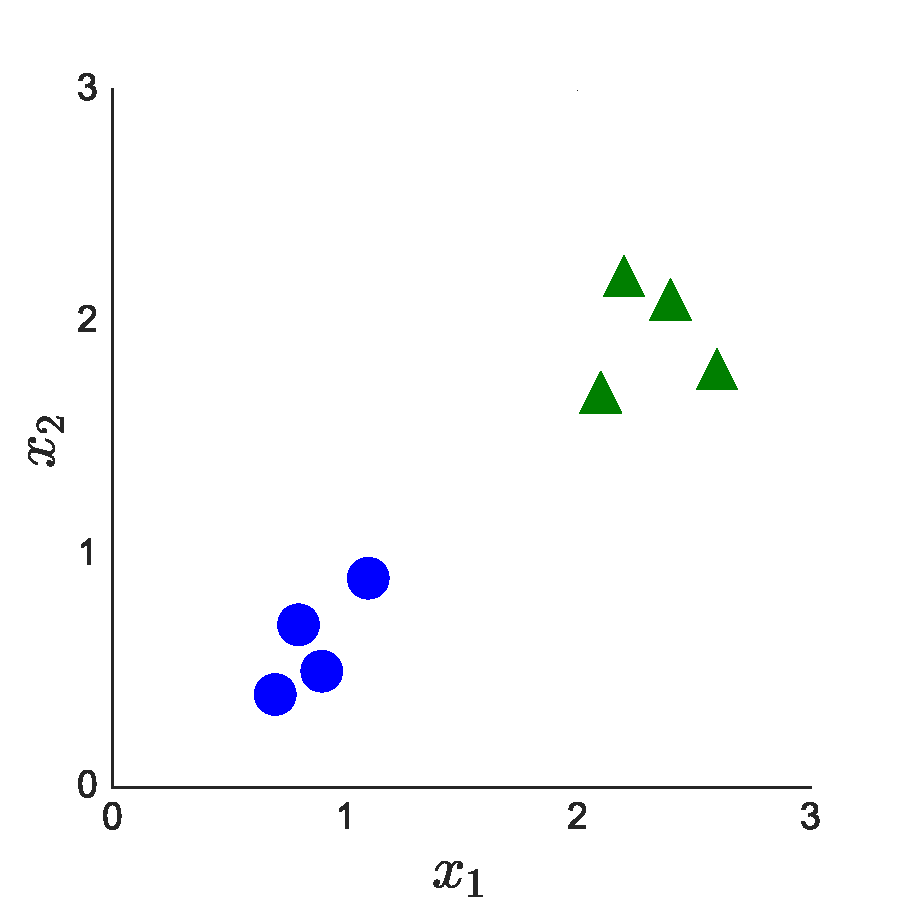
\includegraphics[scale=0.45]{logreg_eg6_binary_eg_data.pdf} 
   		\caption[]{Binary Classification}
   		\label{logreg_eg6_binary_eg_data.pdf}
	\end{subfigure}
	\begin{subfigure}[t]{0.45\textwidth}
   		\centering
    		\graphicspath{{./Figures/}}
   		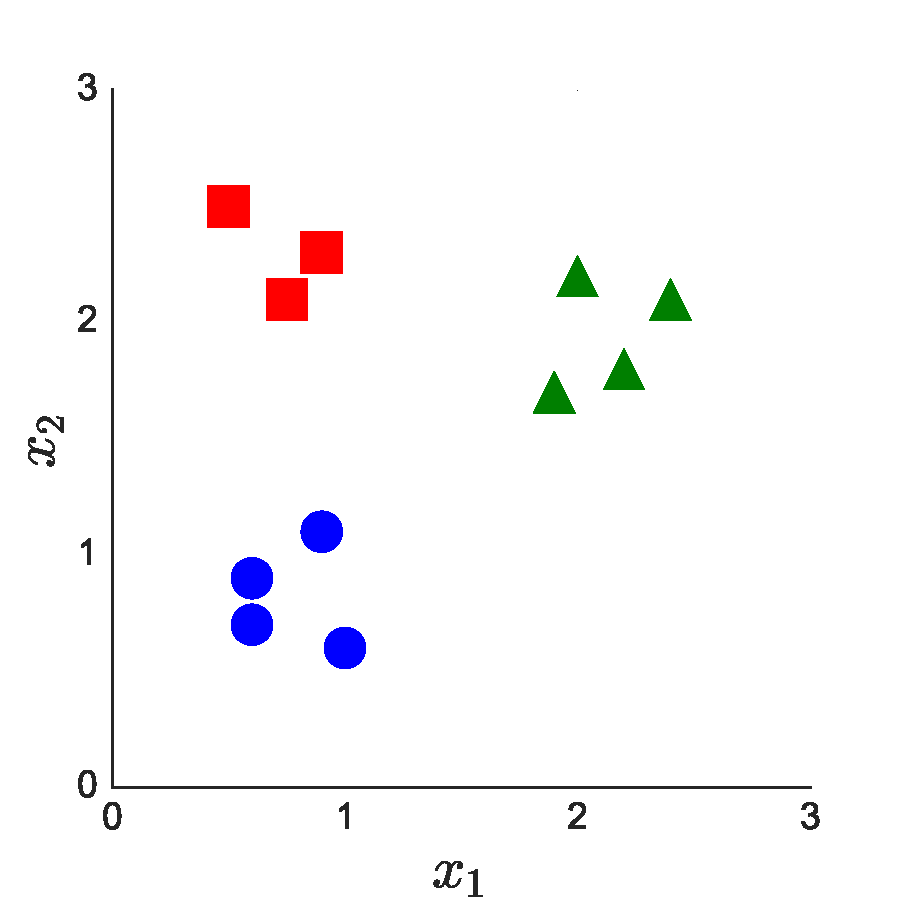
\includegraphics[scale=0.45]{logreg_eg6_multiclass_eg_data.pdf} 
   		\caption[]{Multiclass Classification}
   		\label{logreg_eg6_multiclass_eg_data.pdf}
	\end{subfigure}
	\caption[]{Examples of binary and multiclass classification.}
%	\label{}
\end{figure}
Previously, for a binary classification problem, our data looked like the data in Figure \ref{logreg_eg6_binary_eg_data.pdf}, with multiclass classification, the data looks more like Figure \ref{logreg_eg6_multiclass_eg_data.pdf}.
\begin{figure}[h] %  figure placement: here, top, bottom, or page
	\centering
	\graphicspath{{./Figures/}} %Use this to import an image from a subfolder.
	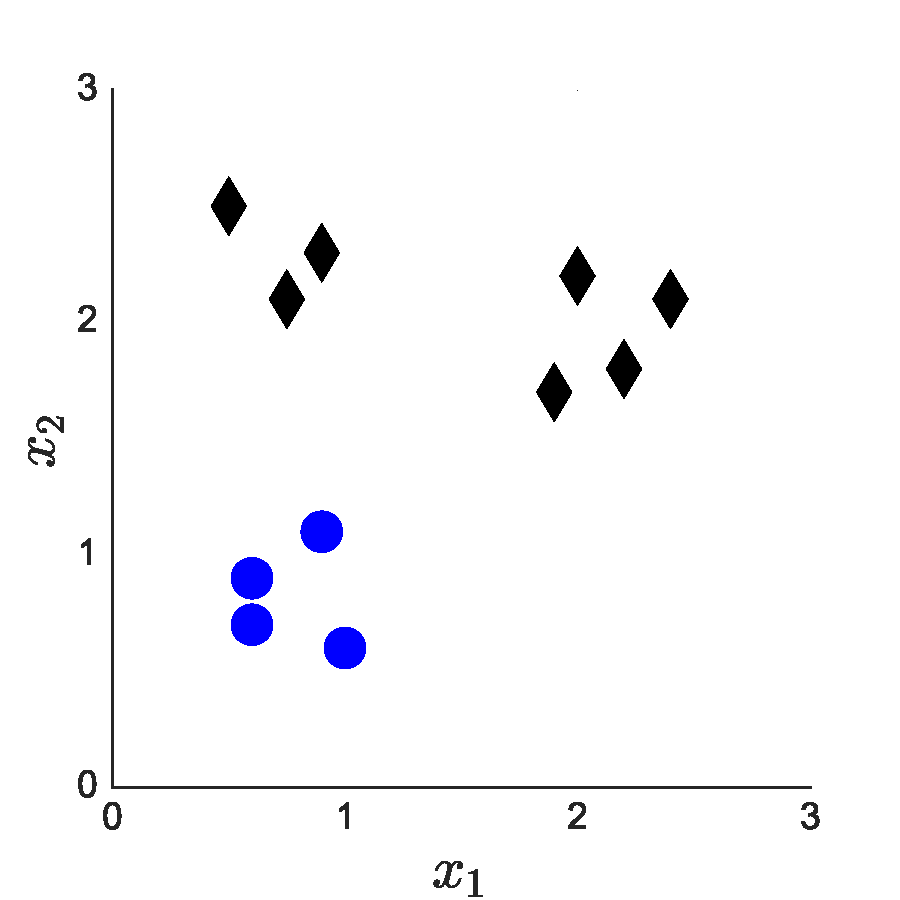
\includegraphics[scale=0.45]{logreg_eg6_multiclass_onevall_step1.pdf} 
	\caption[]{One-vs-all classification. We're selecting one class to be our positive class, and the rest all become the negative class.}
	\label{logreg_eg6_multiclass_onevall_step1.pdf}
\end{figure}

We know how to perform binary classification, but how to we make this work with more classes? We can use the idea of one-vs-all classification.\footnote{This can also be called one-vs-rest classification.} Here's how it works; let's say we have a training set of three classes (such as in Figure \ref{logreg_eg6_multiclass_eg_data.pdf}). What we can do is turn this into three separate binary classification problems.\footnote{If we have $n$ different classes, our problem splits into $n+1$ different binary classification problems.This is because the vector $\vec{y}$ starts at index $0$, so $\left|\left|\vec{y}\right|\right| = n+1$.} Start by picking a class, say the blue circles, and make it our positive class; then lump all the other data into the negative class (see Figure \ref{logreg_eg6_multiclass_onevall_step1.pdf}).

We fit a classifier to this, called $h_\theta^{\left(1\right)}\left(x\right)$. We then do this for the two other classes, and fit them to logistic regression classifiers $h_\theta^{\left(2\right)}\left(x\right)$ and $h_\theta^{\left(3\right)}\left(x\right)$. Here, we've fit three classifiers
\begin{equation}
h_\theta^{\left(i\right)}\left(x\right) = P\left(y=i | x; 0\right)	~~\mbox{\;\;\;\;\;\;\;\;\;\; for } i = \{1, 2, 3\}
\end{equation}
that are trying to estimate the probability that $y$ is equal to class $i$, given $x$ and parameterized by $\theta$. So  $h_\theta^{\left(i\right)}\left(x\right)$ is trying to estimate the probability that a data point is of class $i$. 

For a new input $x$, to make a prediction, we pick the class $i$ that maximizes 
\begin{equation}
\max_i  h_\theta^{\left(i\right)}\left(x\right)
\end{equation}
and this tells us which class to assign the new input to. 





\section{Regularization}
For the two machine learning algorithms we've seen so far, they tend to work pretty well. But when applied to specific datasets, they can run into a problem called overfitting, and this can cause them to perform very poorly. We're going to discuss a little more detail about this problem, and then go into ways to ameliorate it and increase our algorithm performance. Let's plot some housing data, and then take a look at three potential regressions. 

\begin{figure}[h]
	\centering
	\begin{subfigure}[t]{0.3\textwidth}
   		\centering
    		\graphicspath{{./Figures/}}
  		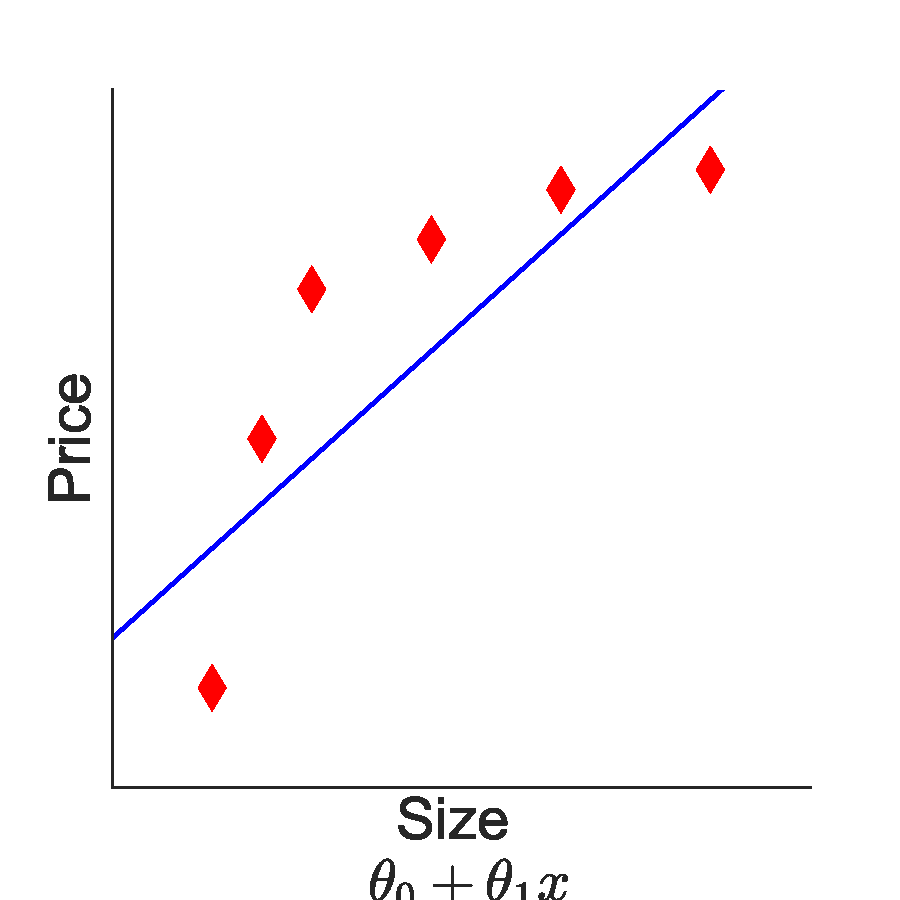
\includegraphics[scale=0.35]{logreg_eg7_housing_data_linreg.pdf} 
   		\caption[]{Linear Regression}
   		\label{logreg_eg7_housing_data_linreg.pdf}
	\end{subfigure}
	\begin{subfigure}[t]{0.3\textwidth}
   		\centering
    		\graphicspath{{./Figures/}}
   		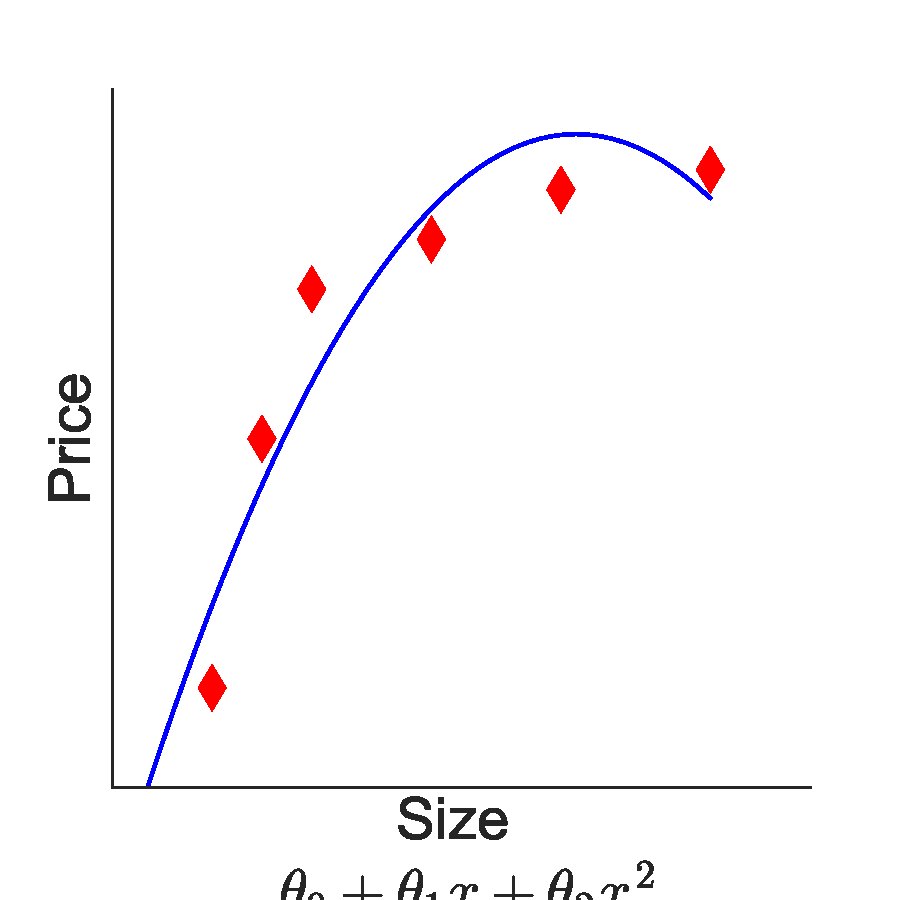
\includegraphics[scale=0.35]{logreg_eg7_housing_data_quadreg.pdf} 
   		\caption[]{Quadratic Regression}
   		\label{logreg_eg7_housing_data_quadreg.pdf}
	\end{subfigure}
	\begin{subfigure}[t]{0.3\textwidth}
   		\centering
    		\graphicspath{{./Figures/}}
   		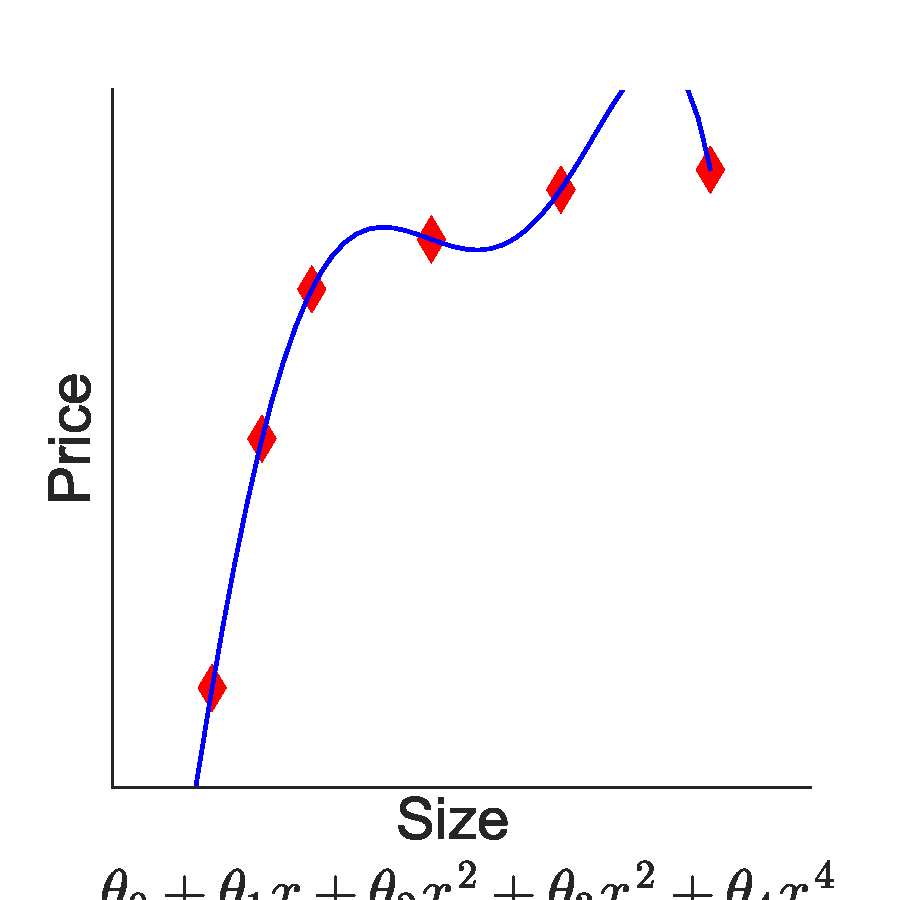
\includegraphics[scale=0.35]{logreg_eg7_housing_data_quadreg_overfit.pdf} 
   		\caption[]{Quadratic Regression with Additional Terms}
   		\label{logreg_eg7_housing_data_quadreg_overfit.pdf}
	\end{subfigure}
	\caption[]{Plots of linear and quadratic regressions with varying amounts of terms (features). }
%	\label{}
\end{figure}

Figure \ref{logreg_eg7_housing_data_linreg.pdf} is a linear regression on this data. This is the simplest regression, but looking at the data, it seems pretty clear that this isn't really a good fit. As the size of the house increases, the housing prices seem to plateau after a certain point, whereas the linear regression line keeps increasing. This is known as \textbf{underfitting}, or \textbf{high bias}.\footnote{The term \textit{bias} is somewhat or a historical or technical term. It carries with it the idea that if fitting a straight line to the data, it's as if the algorithm has a preconception (or bias) that the housing prices should vary linearly with their size, despite evidence in the data that this is not the case. Irrespective of the evidence to the contrary, the algorithm fits the data to a straight line, and it ends up not being a very good fit.} Both of these roughly mean that the regression just isn't fitting to the training data very well. In Figure \ref{logreg_eg7_housing_data_quadreg.pdf}, we can fit a quadratic function to the data. This seems to work pretty well, and looks like a better fit than the linear regression. Figure \ref{logreg_eg7_housing_data_quadreg_overfit.pdf} shows what happens when we \textbf{overfit} the line. This is also known as \textbf{high variance}. The curve fits the training set very well, but it particular to the specific training set, so it doesn't work well for any other data set. 

Let's formally define these terms now:
\begin{description}
\item[Overfitting] If we have too many features, the learned hypothesis may fit the training set very well ($J\left(\theta\right) \approx 0$), but fails to generalize to new examples. This is also called high variance. 
\item[Underfitting] This occurs when the form of our hypothesis function maps poorly to the trend of the data. It is usually caused by a function that is too simple or uses too few features. This is also called high bias. 
\end{description}
This apply to both linear and logistic regression. 

So how do we prevent our models from overfitting to the data? For the simple examples where we have one or two features, we can plot the data and determine it that way; but when we start working with data sets that have hundreds of features, this no longer works. We have two main options to address overfitting:
\begin{enumerate}
\item Reduce the number of features
	\begin{itemize}
	\item Manually select which features to keep, or
	\item Use a model selection algorithm (which we'll see later)
	\end{itemize}
\item Regularization
	\begin{itemize}
	\item Keep all the features, but reduce the parameters $\theta_j$
	\end{itemize}
\end{enumerate}
Regularization works well when we have a lot of slightly-useful features. 

\subsection{Cost Function}
If we suspect overfitting in our hypothesis function, we can reduce the weight of some of the terms in our function by increasing their cost. Say we have a hypothesis of the form
$$
h_\theta\left(x\right) = \theta_0 + \theta_1x + \theta_2x^2 + \theta_3x^3 + \theta_4x^4
$$
To reduce the effect of $\theta_3x^3$ and $\theta_4x^4$ without actually getting rid of those features, we instead modify our cost function to something like this
$$
\min_\theta \frac{1}{2m} \sum_{i=1}^m \left(h_\theta \left(x ^{\left(i\right)}\right) - y^{\left(i\right)}\right)^2 + 1000\left(\theta_3\right)^2 + 1000 \left(\theta_4\right)^2
$$
where $1000$ is an arbitrary large number that we chose. This inflates the cost of both $\theta_3$ and $\theta_4$, so to reduce our cost function, we end up reducing the values of $\theta_3$ and $\theta_4$ to near zero. This will greatly reduce the values of $\theta_3x^3$ and $\theta_4x^4$ in our hypothesis function. This usually yields a simpler hypothesis that is less prone to overfitting. 

In a more general sense, having small values for \textit{all} parameters typically decreases the likelihood that we'll overfit our regression. 

To implement regularization, we modify the cost function by adding a regularization term at the end to shrink every parameter, where $\lambda$ is called the regularization parameter. 
\begin{equation}
J_\theta = \frac{1}{2m}\left[ \sum_{i=1}^m \left(h_\theta\left( x^{(i)}\right) - y^{(i)}\right)^2 + \lambda\sum_{j=1}^n \theta_j^2\right]
\end{equation}
By convention, these summations start at $1$, so we don't regularize $\theta_0$. In this equation, the regularization parameter $\lambda$ controls the trade-off between two different goals: fitting the training data well (the first term of the equation), and keeping the parameters small (the regularization term). 

Conceptually, it can be somewhat difficult to see why keeping the parameters small reduces overfitting, but if you program this yourself, you'll see this effect firsthand. What actually happens is that by using the above cost function with regularization, the resulting output of the hypothesis function is smoothed out to reduce overfitting. However, if $\lambda$ is chosen to be too large, it may smooth out the function too much and underfit. For example, if $\lambda \sim 10^{10}$ for our housing data problem, then $\theta_j \to 0$ for $j \neq 0$.This leaves us with a regression that looks like $h_\theta\left(x\right) = \theta_0$, meaning our hypothesis is just a horizontal line. 


\subsection{Regularized Linear Regression}
We've previously looked at two algorithms for linear regression: one based on gradient descent, and one based on the normal equation. Now, we'll take these two algorithms and generalize them to regularized linear regression. Here is our cost function
\begin{equation}
J_\theta = \frac{1}{2m}\left[ \sum_{i=1}^m \left(h_\theta\left( x^{(i)}\right) - y^{(i)}\right)^2 + \lambda\sum_{j=1}^n \theta_j^2\right]
\end{equation}
and our goal is to get
\begin{equation}
\min_\theta J\left(\theta\right)
\end{equation}

\subsubsection{Gradient Descent}
Our standard gradient descent algorithms looks something like this:

\textbf{Repeat \{}
$$
\theta_j := \theta_j - \alpha \frac{1}{m} \sum_{i=1}^m \left( h_\theta\left(x^{(i)}\right) - y^{(i)}\right) x_j^{(i)} ~~\mbox{\;\;\;\;\;\;\;\;\;\; for } j = 0, 1, 2, \dots, n
$$
\textbf{\}} \\

\noindent To make this easier, we're just going to write the update for $\theta_0$ separately.

\textbf{Repeat \{}
\begin{subequations}
\begin{align}
\theta_0 &:= \theta_0 - \alpha \frac{1}{m} \sum_{i=1}^m \left( h_\theta\left(x^{(i)}\right) - y^{(i)}\right) x_0^{(i)} \\
\theta_j &:= \theta_j - \alpha \frac{1}{m} \sum_{i=1}^m \left( h_\theta\left(x^{(i)}\right) - y^{(i)}\right) x_j^{(i)} ~~\mbox{\;\;\;\;\;\;\;\;\;\; for } j = 1, 2, \dots, n \label{chaplogreg-sectregular-subsect-linreg-graddesc-oldeqtn}
\end{align}
\end{subequations}
\textbf{\}} \\
Now, we want to modify these equations to include our new regularization parameter. The $\theta_0$ equation stays the same since we don't regularize $\theta_0$, but equation \ref{chaplogreg-sectregular-subsect-linreg-graddesc-oldeqtn} becomes
\begin{subequations}
\begin{align}
\theta_0 &:= \theta_0 - \alpha \frac{1}{m} \sum_{i=1}^m \left( h_\theta\left(x^{(i)}\right) - y^{(i)}\right) x_0^{(i)} \\
\theta_j &:= \theta_j - \alpha \left[\frac{1}{m} \sum_{i=1}^m \left( h_\theta\left(x^{(i)}\right) - y^{(i)}\right) x_j^{(i)} + \frac{\lambda}{m}\theta_j \right] ~~\mbox{\;\;\;\;\;\;\;\;\;\; for } j = 1, 2, \dots, n \label{chaplogreg-sectregular-subsect-linreg-graddesc-neweqtn}
\end{align}
\end{subequations}
If you do the calculus out, you can prove that the large term in brackets in equation \ref{chaplogreg-sectregular-subsect-linreg-graddesc-neweqtn} is the partial derivative of the new $J\left(\theta\right)$ with the regularization term. 
$$
\frac{\partial}{\partial \theta_j} J\left(\theta\right)
$$
With some manipulation, we can rewrite our update rule as
\begin{equation}
\theta_j := \theta_j\left(1 - \alpha\frac{\lambda}{m}\right) - \alpha\frac{1}{m}\sum_{i=1}^m \left(h_\theta\left(x^{(i)}\right) - y^{(i)}\right) x_j^{(i)}
\end{equation}
where in the first term in the equation, the value $1 - \alpha\frac{\lambda}{m}$ will always be less than one. Intuitively, the term that's always less than one will serve to reduce $\theta_j$ by a small amount, and the other term is actually exactly the same as our previous gradient descent algorithm before we introduced regularization. 

\subsubsection{The Normal Equation}
Gradient descent was just one of the two algorithms we've explored as a solution to linear regression; the second algorithm was based on the normal equation. With the normal equation, we crafted the design matrix $X$ where each row corresponds to a separate training example, and we have an $m$-dimensional vector $\vec{y}$ that contains our labels. 
$$
X = \left[\begin{array}{c}
\left(x^{(1)}\right)^\intercal \\ \left(x^{(2)}\right)^\intercal \\ \vdots \\ \left(x^{(m)}\right)^\intercal
\end{array}\right] ~~\mbox{ \;\;\;\;\;\;\;\;\;\; }~~ \vec{y} = \left[\begin{array}{c} y^{(1)} \\ y^{(2)} \\ \vdots \\ y^{(m)} \end{array}\right]
$$
where we calculated the vector $\vec{\theta}$ as 
$$
\vec{\theta} = \left( X^\intercal X\right)^{-1} X^\intercal \vec{y}
$$
This minimized the unregularized cost function $J\left(\theta\right)$. To add in regularization, we add another term inside the parentheses
\begin{equation}
\vec{\theta} = \left( X^\intercal X + \lambda L \right)^{-1} X^\intercal \vec{y}
\end{equation}
where the matrix $L$ is a diagonal matrix\footnote{In linear algebra, a diagonal matrix is a matrix (usually a square matrix) in which the off-diagonal elements are all zero. The main diagonal entries themselves may or may not be zero.} given by:
\begin{equation}
L = \left[\begin{array}{cccccc}
0 &  &  &  &  &  \\
 & 1 & & & & \\
& & 1 & & & \\
& & & 1 & & \\
& & & & \ddots & \\
& & & & & 1
\end{array}\right]
\end{equation}
The matrix $L$ has $0$ in it's top left spot, then $1$'s down the diagonal and zeros everywhere else. It has dimensions $\left(n+1\right) \times \left(n+1\right)$. Intuitively, this is the identity matrix (sans $x_0$), multiplied by a single number $\lambda \in \mathbb{R}$.

Recall that if the number of examples $m \leq$ the number of features $n$, then $X^\intercal X$ is non-invertible.\footnote{A non-invertible square matrix is also called singular or degenerate.} We got around this programatically by using the pseudoinverse. Fortunately, regularization also takes care of this for us as well. As long as $\lambda \in \mathbb{R}_{>0}$ is strictly greater than zero, then $X^\intercal X + \lambda L$ will be strictly invertible. 


\subsection{Regularized Logistic Regression}





\section{Python Labs: Coding Logistic Regression in Python}
\section{Homework}




























